\newpage
\subsection{Term-by-Term Enstrophy Transport Evaluation}
The following results show the time evolution of both the enstrophy and
kinetic energy transport terms for a simulation with the following Dynamic
Smagorinsky coefficient

\begin{equation}
    C_{DS} = 
    \begin{cases}
        0.0         &   \text{for $t  < t^{\ast} = 30.0$} \\
        0.65        &   \text{for $t \geq t^{\ast} = 30.0 $} \\
    \end{cases}
\end{equation}
Furthermore the simulation was performed on a 32x32x32 grid for 5k timsteps. 
From figs~(\ref{fig:enst-1330}-\ref{fig:ke-4750}) we can see the following
results:
\begin{enumerate}
    \item The further into the blowup region the more local the blowup
        becomes, as well as the more similar the enstrophy and the kinetic
        energy fields become.
        
    \item The main contributors in the enstrophy transport are
        $\Pi_{\Omega}$ and $P_{\Omega}$.

    \item The main contributors in the kinetic energy are $A$, $C$, $P$. 

    \item It is somewhat hard to see from these results, and I think it is
        easier in the average value plots, that the enstrophy does blowup
        faster then the kinetic energy. I think that this makes sense we
        had speculated that the blowup is local process. Furthermore, since
        there are higher order derivatives in the enstrophy transport
        equation, compared to the kinetic energy, we see more effects of
        the smaller scale effects of $\tau_{ij}$ which could also be
        increasing the rate of blowup in the enstrophy transport.

    \item When comparing the enstrophy and kinetic transport equations it
        clear that the enstrophy transport is much more local compared to
        the kinetic energy. We can see that transport of kinetic energy is
        a lot more spread out across the domain as compared to the
        enstrophy that has very high local values.

\end{enumerate}


\subsection{Results for $C_{DS}=0.0$}
The following results are for a run with the following input conditions:
\begin{longtable}[c]{A{3.0cm}  A{3.0cm}}
    \caption{Input list for $C_{DS}=0$ test}    \\  \hline
        \textbf{Parameter}      &       \textbf{Value}      \\  \hline
    \endfirsthead
    \caption{Input list for $C_{DS}=0$ test~(continued)}    \\  \hline
        \textbf{Parameter}      &       \textbf{Value}      \\  \hline
    \endhead
        $N$                 &   64      \\
        $t_{final}$         &   100.0   \\
        $C_{DS}$            &   0.0     \\
        $C_{BS}$            &   1.0     \\
\end{longtable}

\begin{figure}[H]
    \includegraphics[height=0.4\textheight]{media/run-cds-00/average-ke-cds-00}
    \caption{Average kinetic energy versus simulation time}
\end{figure}

\begin{figure}[H]
    \includegraphics[height=0.4\textheight]{media/run-cds-00/A-term-enstrophy}
    \caption{$A_{\Omega}$ results at $z=32$}
\end{figure}

\begin{figure}[H]
    \includegraphics[height=0.4\textheight]{media/run-cds-00/C-term-enstrophy}
    \caption{$B_{\Omega}$ results at $z=32$}
\end{figure}

\begin{figure}[H]
    \includegraphics[height=0.4\textheight]{media/run-cds-00/D-term-enstrophy}
    \caption{$D_{\Omega}$ results at $z=32$}
\end{figure}

\begin{figure}[H]
    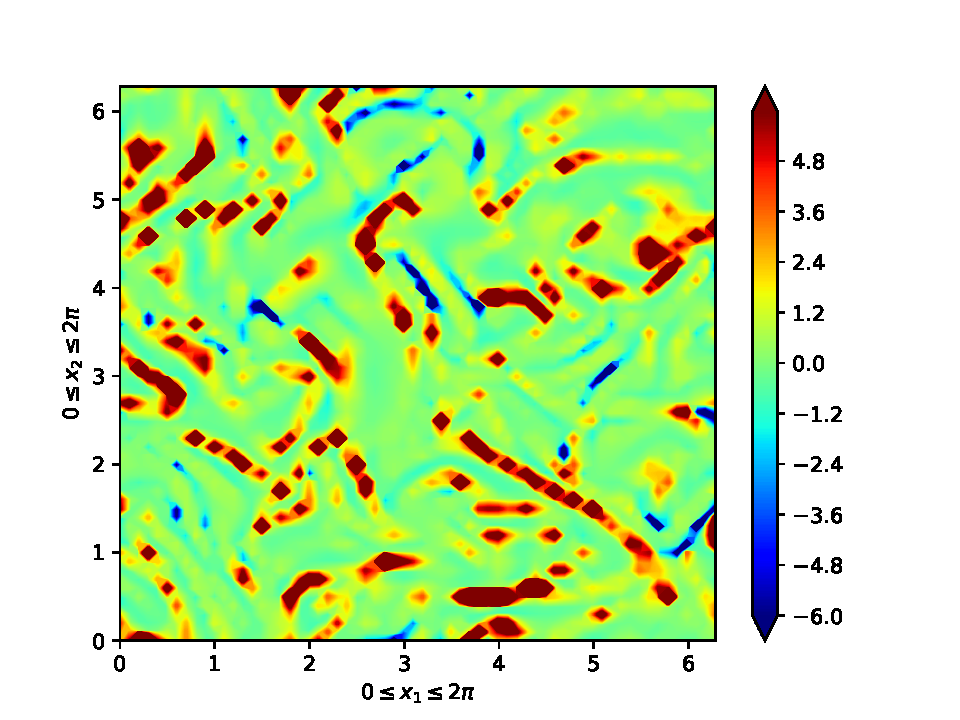
\includegraphics[height=0.4\textheight]{media/run-cds-00/SGS-transport-term-enstrophy}
    \caption{$\Pi_{\Omega}$ results at $z=32$}
\end{figure}

\begin{figure}[H]
    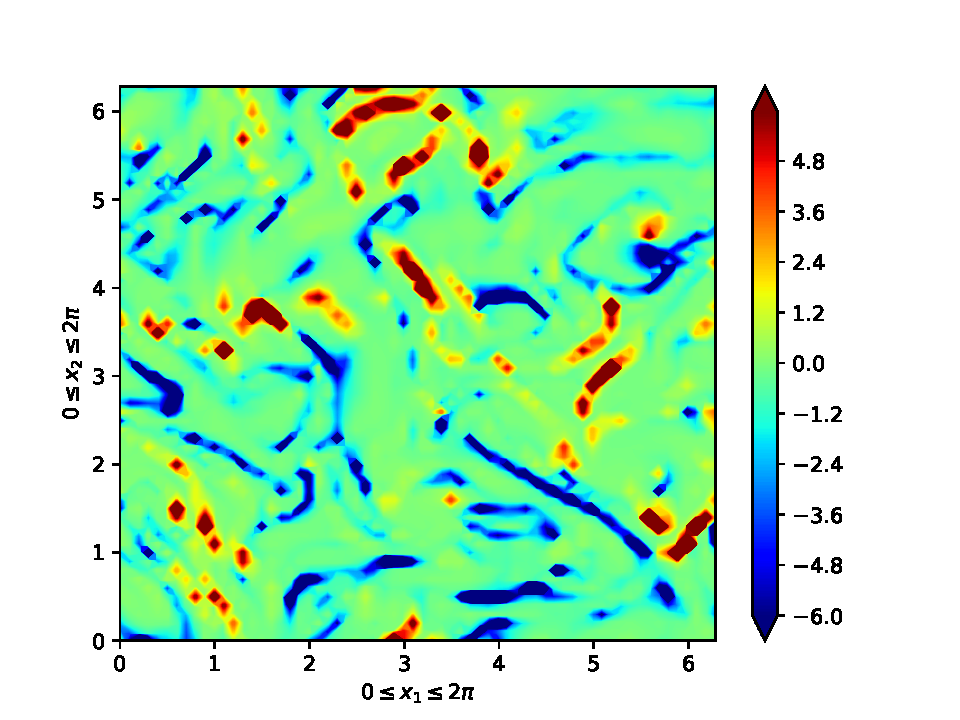
\includegraphics[height=0.4\textheight]{media/run-cds-00/SGS-production-term-enstrophy}
    \caption{$P_{\Omega}$ results at $z=32$}
\end{figure}

